% This is lnbip.tex the demonstration file of the LaTeX macro package for
% Lecture Notes in Business Information Processing from Springer-Verlag.
% It serves as a template for authors as well.
% version 1.0 for LaTeX2e
%
\documentclass[lnbip]{svmultln}
%
\usepackage{makeidx}  % allows for indexgeneration
% \makeindex          % be prepared for an author index
%
\usepackage{graphics}
\begin{document}
%
\mainmatter              % start of the contribution
%
\title{An Multi Agent System for Argumentation}
\subtitle{Research Report}
%
\titlerunning{Argumentation MAS}  
% abbreviated title (for running head)
% also used for the TOC unless
% \toctitle is used
%
\author{Alexandru Sorici \and Alin Danciu \and Tudor Berariu}
%
\authorrunning{A. Sorici, A. Danciu, T. Berariu}
% abbreviated author list (for running head)
%
%%%% list of authors for the TOC (use if author list has to be modified)
\tocauthor{Alexandru Sorici, Alin Danciu, Tudor Berariu}
%
\institute{Faculty of Automatic Control and Computer Science, \\ University "Politehnica" of Bucharest, Romania}

\maketitle              % typeset the title of the contribution

\begin{abstract}        % give a summary of your paper
%abstract to do
% please supply keywords within your abstract
\keywords {natural language processing, machine learning, argumentation, statistical learning, multi agent system}
\end{abstract}
%
\label{cha:chap1}

\section{Introduction}\label{sec:intro}


\subsection{Argumentation in Computer Science}
\par
With regards to computer science, the study of argumentation is crucial in many artificial intelligence and natural language research problems.
\par
For example, in the field of Multi Agent Systems (MAS) reasoning agents need to communicate with each other and apply argumentation-based reasoning mechanisms to resolve the conflicts arising from their different views of goals, beliefs, and actions.
Another example are question answering systems, which deal with finding the correct response to questions like ``Why was this decision taken?'' and therefore integrate the analysis of argumentation as a crucial part of identifying the answer to the questions as well as the pros and cons that make up the answer.
\par
The field of computer-supported collaborative learning (CSCL) has, in particular, been interested in argumentation and how students can benefit from it (Stegmann et al. 2007 - \textit{Facilitating argumentative knowledge construction with computer-supported collaboration scripts};). So-called ``collaborative argumentation'' is viewed as a key way in which students can learn critical thinking, elaboration, and reasoning.
Therefore, it is a crucial point to understand the characteristics and models of argumentation.
\par
Argumentation mining, the subject we are trying to approach, is a new research area that moves between natural language processing, argumentation theory and information retrieval. The aim of argumentation mining is to automatically detect the argumentation of a document and its structure.
\par
Some relevant work in this area has been done by R.M. Palau and M-F Moens in \textit{Argumentation mining: the detection, classification and structure of arguments in text}. In the paper they analyze the main research questions when dealing with argumentation mining and the different methods they have studied and developed in order to successfully confront the challenges of argumentation mining in legal texts.
A more structured approach is taken by Safia ABBAS , Hajime SAWAMURA in \textit{ALES: An Innovative Argument Learning Environment}. The environment uses different mining techniques to manage a highly structured arguments repository.
 \par
Overall, the task of argument extraction from free text is a new and difficult research area, one that will hopefully see a lot of activity in the near future, because the results that can be obtained will be of great use in many related fields of natural language processing.

\section{Argumentation Concepts Overview}
\par A nice overview on argumentation tasks and concepts was given by Douglas Walton in his research reports. The next sections are inspired by his work.
\subsection{Main problems}
\par
There are four tasks undertaken by argumentation:
\begin{description}
\item[identification] which means finding the premises and conclusion fo arguments in a text and fitting that argument in an argumentation scheme;
\item[analysis] which involves the identification of implicit premises or conclusion of arguments (such an argument is called an enthymeme);
\item[evaluation] where the strength of an argument must be determined using a general criteria;
\item[invention] which means constructing new arguments that can be used to prove some conclusion
\end{description}
\subsection{Argument definition}
\par
An argument is a set of statements (propositions), made up of three parts, a conclusion, a set of premises, and an inference from the premises to the conclusion. An argument can be supported by other arguments, or it can be attacked by other arguments, and by raising critical questions about it.
\par
The definition of `argument' relied on so far could be called a minimal inferential definition, and the method of argument diagramming shown so far fits this minimal definition. The boxes represent propositions and the arrows represent inferences from some propositions to others.
\par
The general approach or methodology of argumentation can be described as distinctively different from the traditional approach based on deductive logic. The traditional approach concentrated on a single inference, where the premises and conclusion are designated in advance, and applied formal models like propositional
calculus and quantification theory determine whether the conclusion conclusively follows from the premises. This approach is often called monological.
\par
In contrast, the argumentation approach is called dialogical (or dialectical) in that it looks at two sides of an argument, the pro and the contra. According to this approach, the method of evaluation is to examine how the strongest arguments for and against a particular proposition at issue interact with each other, and in particular how each argument is subject to probing critical questioning that reveals doubts about it. By this dialog process of pitting the one argument against the other, the weaknesses in each argument are revealed, and it is shown which of the two arguments is the stronger.
\subsection{Argument Attack and Refutation}
\par
There are several ways to attack an argument and the easiest way is to ask an appropriate critical question that raises doubt about the acceptability of the argument. When this happens, the argument temporarily defaults until the proponent can respond appropriately to the critical question. Another way to attack an argument is to question one of the premises. A third way to attack an argument is to put forward counter-argument that opposes the original argument, meaning that the conclusion of the opposing argument is the opposite (negation) of the conclusion of the original argument.
\par
A simple way to represent a sequence of argumentation is using a directed graph:
\begin{center}
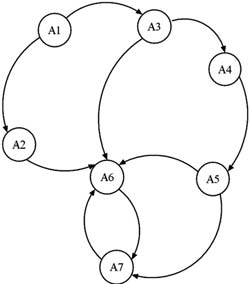
\includegraphics{attack.png}
\end{center}
\subsection{Argumentation Schemes}
\par
Some of the most common schemes are: argument from witness testimony, argument from expert opinion, argument from popular opinion, argument from example, argument from analogy, practical reasoning (from goal to action), argument from verbal classification, argument from sign, argument from sunk costs, argument from appearance, argument from ignorance, argument from cause to effect, abductive reasoning, argument from consequences, argument from alternatives, argument from pity, argument from commitment, ad hominem argument, argument from bias, slippery slope argument, and argument from precedent. Each scheme has a set of critical questions matching the scheme and such a set represents standard ways of critically probing into an argument to find aspects of it that are open criticism.
\subsection{Types of dialog}
There are six types of dialogs:
\begin{description}
\item[Persuasion] generated by a \textbf{Conflict of Opinions} in which each party tries to \textbf{Persuade Other Party} in order to \textbf{Resolve or Clarify Issue}
\item[Inquiry] generated by the \textbf{Need to Have Proof} in which each party tries to \textbf{Find and Verify Evidence} in order to \textbf{Prove (Disprove) the Hypothesis}
\item[Negotiation] generated by a \textbf{Conflict of Interests} in which each party tries to \textbf{Get What He Most Wants} in order to reach a \textbf{Reasonable Settlement Both Can Live With}
\item[Information-Seeking] catalyzed by the \textbf{Need of Information} in which each party \textbf{Acquires or Gives Information} in order to \textbf{Exchange Information}
\item[Deliberation] generated by a \textbf{Deliberation Dilemma or Practical Choice} that is needed in which the participants try to \textbf{Co-ordinate Goals and Actions} in order to \textbf{Decide on Best Available Course of Action}
\item[Eristic] generated by a \textbf{Personal Conflict} in which each party tries to \textbf{Verbally Hit Out at Opponent} in order to \textbf{Reveal Deeper Basis of Conflict}.
\par
On our project we will probably focus on inquiry dialogs.
\end{description}

\section{NLP Aspects Overview}
\par
As stated in the last section the goal of project becomes that of identifying the arguments and the relations that exist between them in a given text. 
As such, our task can be modeled as a classification problem.

\par
As presented previously, there exist a number of models for both the intrinsic structure of a model, as well as for the relations that can hold between them.
The above sections gave a classification of the different types of dialog and argumentation schemes. What is interesting to notice is that each type of dialog supports some argumentation schemes better than others. Thus, having chosen one specific type of dialog, the most relevant argumentation schemes pertaining to that dialog model will be chosen as structure guidelines for our arguments. 
In addition, a Toulmin (S. E. Toulmin. \textit{The Uses of Argument}) based alternative representation of an argument will be considered.

\subsection{Main problems}
\par
Having laid out this model, we are faced with the following challenges of Argumentation Mining: 
\begin{description}
\item Detect all the arguments in a free text (classification problem)
\item Determine argument limits ( segmentation problem)
\item Determine arguments type (complex)
\item Detect argumentation structure (complex)
\end{description}

\par
The Corpus that will be used to for solving the above problems is the one provided by \textit{Arauacaria} (\textit {http://www.arg.dundee.ac.uk/projects/araucariadb/search.php}), which, albeit being not very large, has the advantage of giving annotated argument examples.

\par
In the work by R.M. Palau and M-F Moens:  \textit{Argumentation mining: the detection, classifcation and structure of arguments in text} some solutions to this problems are proposed, some of which we consider to be very useful for our project.
For the problem of argument detection statistical classifiers are employed. In particular, good results can be obtained by using the \textit{maximum entropy model} and \textit{multinomial naive Bayes} classifier which learns a model of the joint probability of an element \textit{x} and its label \textit{y}, \textit{p(x, y)}, and makes its predictions by using Bayes rule to calculate p(y\textbar x) and then selects the most likely label \textit{y}.

\par
For the problem of determining argument limits (grouping of argumentative statements into their corresponding argument) we consider computing the semantic distance between different argumentative units (sentences) and group sentences in one argument if they discuss content that is semantically related. Like in the work of Palau and Moens, we assume that the relatedness of two sentences is a function of the relatedness of their words. We want to employ an ontology based semantic relatedness measure, where the relatedness of words depends on their semantic distances in a lexico-semantic resource such as WordNet.

\par
In the determination of argument types, we also consider the use of statistical classifiers.
The problem here is that while a classification of argumentative statements into premises and conclusions is possible (as shown by Palau and Moens by use of a SVM), the task of determining a specific scheme for an argument is much more challenging. In particular, we have to rely on some domain ontology in order to be able to find semantic features that will allow us to classify the arguments as belonging to a certain scheme.
\par
Extensive use of other NLP tools such as POS taggers will also be made in order to enrich the possible set of features used for classification.

\par
Lastly, the problem of determining the argumentation structure, that is, of relations existing between the arguments, will have to take all the results obtained by the previous steps into consideration. The employed algorithm will make the assumption that the discourse follows the rules of the chosen dialog type and that arguments used within it belong to the appropriate argumentation schemes.

\section{Argumentation System architecture - Module description}
\par
This section gives a general overview of the most important modules of our application. We will give a graphical representation of the main modules and of the relation between them. Afterwards, we will give a more detailed description of each module, highlighting the approaches and algorithms considered for their implementation.

\begin{center}
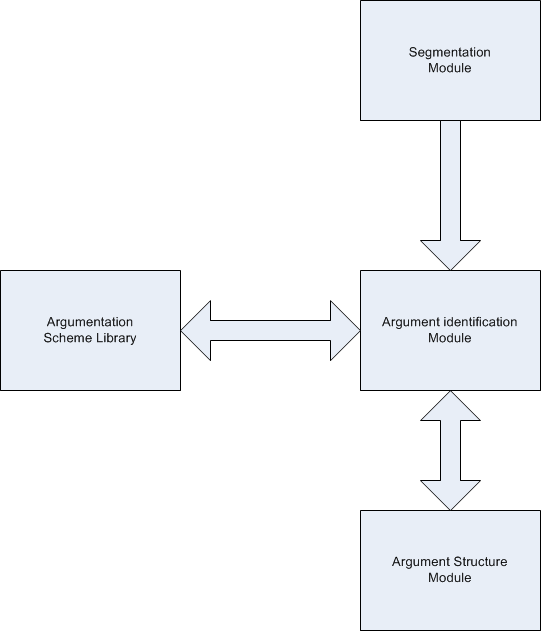
\includegraphics{NLP_Architecture.png}
\end{center}

\subsection{Argument Identification Module}
\par
The Argument Identification Module classifies all sentences into argumentative and non-argumentative utterances. This module’s essential role is to determine which parts of the text are also parts of argument structures.
\par
This module will use a classifier in order to extract argumentative. We will take, most probably, one of the next two options for implementation: a naive Bayes classifier or a maximum-entropy method.
\par
The most important features our classifier will use are:
\begin{description}
\item[Unigrams] Each word in the sentence.
\item[Bigrams] Each pair of successive words.
\item[Trigrams] Each three successive words.
\item[Adverbs] Detected with a part-of-speech (POS) tagger (e.g. QTag 1).
\item[Verbs] Detected with a POS tagger. Only the main verbs (excluding ``to be'', ``to do'' and ``to have'') are considered.
\item[Modal auxiliary] Indicates if a modal auxiliary is present using a POS tagger.
\item[Word couples] All possible combinations of two words in the sentence are considered.
\item[Text statistics] Sentence length, average word length and number of punctuation marks.
\item[Punctuation] The sequence of punctuation marks present in the sentence is used as a feature (e.g. ``:.''). When a punctuation mark occurs more than once in a row, it is considered the same pattern (e.g. two or more successive commas both result in ``,+'').
\item[Key words] Keywords refer to several words or word sequences obtained from a list of terms indicative for argumentation. Examples from the list are ``but'', ``consequently'', and ``because of''.
\end{description}

\subsection{Segmentation Module}
\par
The Argumentation Identification Module uses this module to partition different argumentative sentences (units) into their corresponding arguments, that is, to determine the limits of each individual argument.
\par
In order to achieve this we opt to calculate the semantic distance between the different argumentative units, and group sentences in one argument if they discuss content that is semantically related. As in the work of Palau and Moens, we assume that the relatedness of two sentences is a function of the relatedness of their words.
\par
Given this assumption we take the semantic relatedness of words to be given by their semantic distances in a lexico-semantic resource such as WordNet.
\par
Measures of relatedness are more general in that they can be made across part of speech boundaries, and they are not limited to considering is-a relations.
\par
Several measures of relatedness which are based on the WordNet database can be used.
\begin{itemize}
\item The hso (Hirst and St-Onge, 1998) measures classifies relations in WordNet as having direction, and then establishes the relatedness between two concepts A and B by finding a path that is neither too long nor that changes direction too often. 
\item The lesk (Banerjee and Pedersen, 2003) and vector measures incorporate information from WordNet glosses. The lesk measure finds overlaps between the glosses of concepts A and B, as well as concepts that are directly linked to A and B. 
\item The vector measure (Patwardhan, 2003) creates a co–occurrence matrix for each word used in the WordNet glosses from a given corpus, and then represents each gloss/concept with a vector that is the average of these co–occurrence vectors.
\end{itemize}
\par
WordNet provides modules that implement these measures and that offer a specific API for their usage.
\par
Using these measures we can compute an overall semantic relatedness of the argumentation units. By means of a clustering algorithm that will use the distances given by the above mentioned methods we can then segment sentences into their corresponding arguments (clusters), thus finding the intended argument limits.

\subsection {Argumentation Scheme Library}
\par
The Argumentation Scheme Library contains abstract forms of argument that capture patterns of reasoning. Each argumentation scheme describes the relations between internal parts (the premises and the conclusion) of a complex argument and, also, the set of critical questions that may attack that argument. Chris Reed and Douglas Walton, in their research report ``Towards a Formal and Implemented Model of Argumentation Schemes in Agent Communication'' describe the conventional techniques to handle the structure of argumentation schemes in such way that agents may use them in reasoning and also that communication structures can be built around those schemes.
\par
Example of Argumentation Scheme – Argument from Position To Know:
\begin{description}
\item[Major Premise]: Source \emph{a} is in a position to know about things in a certain subject domain \emph{S} containing proposition \emph{A}.
\item[Minor Premise]: \emph{a} asserts that \emph{A} (in Domain \emph{S}) is true (false).
\item[Conclusion]: \emph{A} is true (false).
\end{description}
This type of argument is defeasible by questioning. Matching the argument from position to know are three critical questions:
\begin{description}
\item[CQ1]: Is \emph{a} in a position to know whether \emph{A} is true (false)?
\item[CQ2]: Is \emph{a} an honest (trustworthy, reliable) source?
\item[CQ3]: Did \emph{a} assert that \emph{A} is true (false)?
\end{description}
\par
Our Argumentation Scheme Library will be trained from Araucaria DB, which contains several real instantiations of argumentation schemes. The representation used is Argument Markup Language, based upon the industry standard XML.

\subsection{Argument Structure Module}
\par
The Argument Identification Module and Segmentation Module were used to distinguish between argumentative and non-argumentative sentences and to group argumentative sentences together into their corresponding argument.
\par
The purpose of this module thus becomes to determine the internal structure of an argument, i.e. the organization of its clauses into conclusions and supporting premises. 
\par
We will consider two possible approaches for this task.
\par
The first relies again on work done by Palau and Moens in Argumentation Mining: The Detection, Classification and Structuring of Arguments in Text and considers the partition of an argument’s units into premises or conclusions.
\par
For each argument, certain features will be determined. The list can comprise features such as:
\begin{description}
\item[Tense of Main Verb]: Tense of the verb from the main clause of the sentence; having as nominal values ``Present'', ``Past'' or ``No Verb''.
\item[History]: The most probable argumentative category of previous and next sentence.
\item[Rhetorical Patterns]: Type of rhetorical pattern occurring on current, previous and next sentences (e.g. ``however,'')
\item[Argumentative Patterns]: Type of argumentative pattern occurring in sentence
\end{description}
A SVM (Support Vector Machine) based algorithm that uses these features will then be used to classify the sentences of an argument into either premises or conclusions.
\par
The second approach is an extension of the first one. Rather than just distinguishing between premise and conclusion, this approach tries to map the argument’s structure onto one or several argumentation schemes. 
\par
The definition and format of these schemes is provided by the Argumentation Scheme Library module. 
\par
Making use of more extended features, that will also include the ones listed above, our SVM based algorithm will this time be trained to distinguish between different argumentation schemes. 
\paragraph*{The role of the segmentation module is that to partition different argumentative sentences (units) into their corresponding arguments, that is, to determine the limits of each individual argument.}
\paragraph*{As presented in the description of the NLP module capabilities, we opt to calculate the semantic distance between the different argumentative units, and group sentences in one argument if they discuss content that is semantically related.}
\paragraph*{The module receives a list of argumentative sentences as its input. It then uses a word tokenizer to split the sentences into lists of words. Stopwords such as "the", "in", "with" etc. are removed before going to the next step.}
\paragraph*{We assume the semantic relatedness of words to be given by their semantic distances in a lexico-semantic resource such as WordNet. We use the lin similarity measure to compute the relatedness of two synsets. As each word in a sentence can have several senses, one would first have to go through a word sense disambiguation process to determine the most probable meaning. As this process is time-consuming, the current approach employs the use of the most common sense, as defined by WordNet, for each word we encounter.}
\paragraph*{Using the lin similarity we compute a word similarity matrix between every pair of words, one from each sentence.}
\paragraph*{To compute the estimated similarity between two sentences we then use the following method. Given two sentences A and B, for each word from sentence A we compute the most similar word from sentence B, as given by the previously computed matrix.}

\[ b^* = arg \max_b Sim(a,b) \]

\paragraph*{In a similar manner, for each word in sentence B we compute the most similar word from sentence A.}

\[ a^* = arg \max_a Sim(a,b) \]

\paragraph*{Afterwards the similarity between sentences A and B is given by}
\[ ( \sum{a^*} + \sum{b^*}) / (2 * (\mid A\mid + \mid B \mid ) \]
\paragraph*{The above process yields a sentence similarity matrix. This matrix is used as an input to a hierarchical clustering algorithm. We take an empirically determined cutoff distance of 0.875 to cut the resulting cluster dendrogram at the corresponding depth. This results in a list of sentence clusters, each of which contains the components of an individual argument.}
\paragraph*{•}
\paragraph*{Here is a simple example. The initial text:}
\paragraph*{\emph{``It is well established that if any statement is made on the floor of the House by a Member or Minister which another Member believes to be untrue, incomplete or incorrect, it does not constitute a breach of privilege.  In order to constitute a breach of privilege or contempt of the House, it has to be proved that the statement was not only wrong or misleading but it was made deliberately to mislead the House.  A breach of privilege can arise only when the Member or the Minister makes a false statement or an incorrect statement willfully, deliberately and knowingly.    On a perusal of the comments of the Ministers in the matter, I am satisfied that there has been no misleading of the House by them as alleged by the Member.   I have accordingly disallowed the notice of question of privilege.  Copies of the comments of the Ministers have already been made available to Dr. Raghuvansh Prasad Singh.''}}
\paragraph*{The determined word lists:}
\begin{description}
\item[L1:][u`It', u`well', u'established', u'statement', u'made', u'floor', u'House', u'Member', u'Minister',u'another', u'Member', u'believes', u'untrue', u'incomplete', u'incorrect', u'constitute', u'breach', u'privilege']
\item[L2:] [u'In', u'order', u'constitute', u'breach', u'privilege', u'contempt', u'House', u'proved', u'statement', u'wrong', u'misleading', u'made', u'deliberately', u'mislead', u'House']
\item[L3:] [u'A', u'breach', u'privilege', u'arise', u'Member', u'Minister', u'makes', u'false', u'statement', u'incorrect', u'statement', u'wilfully', u'deliberately', u'knowingly']
\item[L4:] [u'On', u'perusal', u'comments', u'Ministers', u'matter', u'I', u'satisfied', u'misleading', u'House', u'alleged', u'Member']
\item[L5:] [u'I', u'accordingly', u'disallowed', u'notice', u'question', u'privilege']
\item[L6:] [u'Copies', u'comments', u'Ministers', u'already', u'made', u'available', u'Dr', u'Raghuvansh', u'Prasad', u'Singh']
\end{description}
\paragraph*{The (simmetric) sentence similarity matrix:}
\begin{center}
  \begin{tabular}{ | l | c | c | c | c | c | c | }
    \hline
	& \emph{1} & \emph{2} & \emph{3} & \emph{4} & \emph{5} & \emph{6} \\ \hline
    \emph{1} & 1.00 & 0.24 & 0.24 & 0.19 & 0.10 & 0.13  \\ \hline
	\emph{2} & 0.24 & 1.00 & 0.21 & 0.19 & 0.14 & 0.10  \\ \hline
	\emph{3} & 0.24 & 0.21 & 1.00 & 0.16 & 0.13 & 0.11  \\ \hline
	\emph{4} & 0.19 & 0.19 & 0.16 & 1.00 & 0.13 & 0.12  \\ \hline
	\emph{5} & 0.10 & 0.14 & 0.13 & 0.13 & 1.00 & 0.06  \\ \hline
	\emph{6} & 0.13 & 0.10 & 0.11 & 0.12 & 0.06 & 1.00  \\ \hline
  \end{tabular}
\end{center}
\paragraph*{The resulting sentence clustering (only the indexes of the sentences are show):}
\[ [[5], [4, 3, 1, 0, 2]] \]
\paragraph*{We can see that sentences 1-5 belong to one argument and sentence 6, which is actually non-argumentative, this being only an illustrative example, belongs to a separate cluster.}
\paragraph*{The current method yields some promising results, but there is still room for improvement, especially in the process of determining word similarities, where we hope to be able to implement a more advanced measurement solution. In particular, the Lin measure can only compute the similarity between words which have the same part of speech (noun, verb etc). The lesk or gloss-vector measures, which we will try to implement in future developments can cross these boundaries and are not limited by is-a relations.}
%
%%
%% ---- Bibliography ----
%%
%\begin{thebibliography}{5}
%
%\bibitem{smit:wat} Smith, T.F., Waterman, M.S.: Identification of Common Molecular
%Subsequences. J. Mol. Biol. 147, 195--197 (1981)
%
%\bibitem{mes} May, P., Ehrlich, H.C., Steinke, T.: ZIB Structure Prediction Pipeline:
%Composing a Complex Biological Workflow through Web Services. In: Nagel,
%W.E., Walter, W.V., Lehner, W. (eds.) Euro-Par 2006. LNCS, vol. 4128,
%pp. 1148--1158. Springer, Heidelberg (2006)
%
%\bibitem{fos:kes} Foster, I., Kesselman, C.: The Grid: Blueprint for a New Computing
%Infrastructure. Morgan Kaufmann, San Francisco (1999)
%
%\bibitem{cff} Czajkowski, K., Fitzgerald, S., Foster, I., Kesselman, C.: Grid
%Information Services for Distributed Resource Sharing. In: 10th IEEE
%International Symposium on High Performance Distributed Computing, pp.
%181--184. IEEE Press, New York (2001)
%
%\bibitem{fos:kes:2} Foster, I., Kesselman, C., Nick, J., Tuecke, S.: The Physiology of the
%Grid: an Open Grid Services Architecture for Distributed Systems
%Integration. Technical report, Global Grid Forum (2002)
%
%\bibitem{url} National Center for Biotechnology Information, http://www.ncbi.nlm.nih.gov
%
%\end{thebibliography}
%
\end{document}
